\documentclass[twoside]{article}
\setlength{\oddsidemargin}{0.25 in}
\setlength{\evensidemargin}{-0.25 in}
\setlength{\topmargin}{-0.6 in}
\setlength{\textwidth}{6.5 in}
\setlength{\textheight}{8.5 in}
\setlength{\headsep}{0.75 in}
\setlength{\parindent}{0 in}
\setlength{\parskip}{0.1 in}

\usepackage{graphicx}
\usepackage{url}

%
% The following commands sets up the lecnum (lecture number)
% counter and make various numbering schemes work relative
% to the lecture number.
%
\newcounter{lecnum}
\renewcommand{\thepage}{\thelecnum-\arabic{page}}
\renewcommand{\thesection}{\thelecnum.\arabic{section}}
\renewcommand{\theequation}{\thelecnum.\arabic{equation}}
\renewcommand{\thefigure}{\thelecnum.\arabic{figure}}
\renewcommand{\thetable}{\thelecnum.\arabic{table}}
\newcommand{\dnl}{\mbox{}\par}

%
% The following macro is used to generate the header.
%
\newcommand{\lecture}[4]{
  \pagestyle{myheadings}
  \thispagestyle{plain}
  \newpage
  \setcounter{lecnum}{#1}
  \setcounter{page}{1}
  \noindent
  \begin{center}
  \framebox{
     \vbox{\vspace{2mm}
   \hbox to 6.28in { {\bf COMPSCI~630~~~Systems
                       \hfill Spring 2017} }
      \vspace{4mm}
      \hbox to 6.28in { {\Large \hfill Lecture #1: #2  \hfill} }
      \vspace{2mm}
      \hbox to 6.28in { {\it Lecturer: #3 \hfill Scribe(s): #4} }
     \vspace{2mm}}
  }
  \end{center}
  \markboth{Lecture {#1}: #2}{Lecture {#1}: #2}
  \vspace*{4mm}
}

%
% Convention for citations is authors' initials followed by the year.
% For example, to cite a paper by Leighton and Maggs you would type
% \cite{LM89}, and to cite a paper by Strassen you would type \cite{S69}.
% (To avoid bibliography problems, for now we redefine the \cite command.)
%
\renewcommand{\cite}[1]{[#1]}

% \input{epsf}

%Use this command for a figure; it puts a figure in wherever you want it.
%usage: \fig{NUMBER}{FIGURE-SIZE}{CAPTION}{FILENAME}
\newcommand{\fig}[4]{
           \vspace{0.2 in}
           \setlength{\epsfxsize}{#2}
           \centerline{\epsfbox{#4}}
           \begin{center}
           Figure \thelecnum.#1:~#3
           \end{center}
   }

% Use these for theorems, lemmas, proofs, etc.
\newtheorem{theorem}{Theorem}[lecnum]
\newtheorem{lemma}[theorem]{Lemma}
\newtheorem{proposition}[theorem]{Proposition}
\newtheorem{claim}[theorem]{Claim}
\newtheorem{corollary}[theorem]{Corollary}
\newtheorem{definition}[theorem]{Definition}
\newenvironment{proof}{{\bf Proof:}}{\hfill\rule{2mm}{2mm}}

% Some useful equation alignment commands, borrowed from TeX
\makeatletter
\def\eqalign#1{\,\vcenter{\openup\jot\m@th
 \ialign{\strut\hfil$\displaystyle{##}$&$\displaystyle{{}##}$\hfil
     \crcr#1\crcr}}\,}
\def\eqalignno#1{\displ@y \tabskip\@centering
 \halign to\displaywidth{\hfil$\displaystyle{##}$\tabskip\z@skip
   &$\displaystyle{{}##}$\hfil\tabskip\@centering
   &\llap{$##$}\tabskip\z@skip\crcr
   #1\crcr}}
\def\leqalignno#1{\displ@y \tabskip\@centering
 \halign to\displaywidth{\hfil$\displaystyle{##}$\tabskip\z@skip
   &$\displaystyle{{}##}$\hfil\tabskip\@centering
   &\kern-\displaywidth\rlap{$##$}\tabskip\displaywidth\crcr
   #1\crcr}}
\makeatother

% **** IF YOU WANT TO DEFINE ADDITIONAL MACROS FOR YOURSELF, PUT THEM HERE:



% Some general latex examples and examples making use of the
% macros follow.

\begin{document}

%FILL IN THE RIGHT INFO.
%\lecture{**LECTURE-NUMBER**}{**DATE**}{**LECTURER**}{**SCRIBE**}
\lecture{6}{February 10}{Emery Berger}{Sam Baxter, Divyesh Harit}

\section{Review of Memory Hierarchy}

\begin{center}
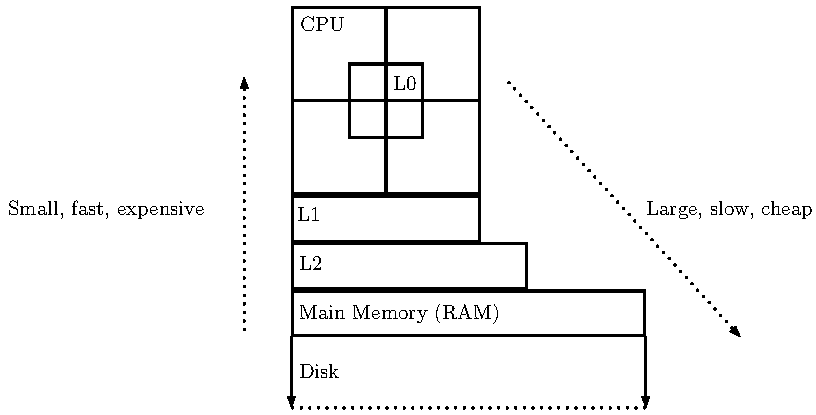
\includegraphics[scale=.6]{hierarchy.pdf}
\end{center}

The memory hierarchy is a series of memories, growing in storage capacity and
memory access latency as distance from the CPU increases. Modern computer
architectures typically have a series of caches built into the CPU (L0, L1, L2,
etc.), followed by RAM, and then by disk.

Access to data stored on disk takes orders of magnitudes longer (in CPU cycles)
than closer memories, which begs the question of how network latencies are
tolerable. Memory access latencies are measured in CPU cycles to retrieve the
first byte of data requested. When accessing many bytes sequentially stored, we
can \emph{prefetch} the remaining bytes while we wait for the first byte to
arrive, hiding the latency so that when the first byte arrives, the rest
immediately follow.

\subsection{Locality}
\textbf{Temporal Locality} refers to the reuse of specific data within a
small window of time. In other words, data has high temporal locality if when it
is accessed, it is likely to be accessed again soon.

\textbf{Spacial Locality} refers to the use of data within relatively close
storage locations from each other.

High temporal and/or spacial locality lend themselves to increased performance
due to caches by hiding the latency of memory accesses by keeping things often
or likely to be used in low-latency caches. Memory that exhibits low locality
leads to cache misses on memory accesses, incurring overhead and degredating
performance of caches.

Ways to lower cache "miss" rate include maintaining good spatial/temportal
locality, or to use bigger caches.

\section{Cache Replacement Policies}

Cache performance is determined by the rate of cache hits and misses. Common
reasons for misses are:
\begin{itemize}
    \item \textbf{Compulsory Misses} - The data has not been accessed previously
    \item \textbf{Capacity Misses} - The data previously resided in cache, but
        has been evicted due to space capacity.
\end{itemize}
Cache misses degrade performance and miss rates are subject to how we evict data
from caches, known as the \textbf{Cache Replacement Policy}.

\subsection{LRU - Least Recently Used}
LRU caches evict the oldest cache entry when capacity has been reached and a
cache miss occurs.

\subsection{MRU - Most Recently Used}
MRU caches evict the newest cache entry. This seems counterintuitive, and is
rarely used in systems.

\subsection{RAND - Random}
RAND caches nondeterministically evict a random entry on cache misses. It
maintains no state information or counter. It can be shown that RAND and LRU
converge in the worst-case. RAND is actually desirable in some scenarios, such
as when many entries are reused often, and a small number have recently but
infrequently been used. A common and popular example is its usage in ARM
architecture.

\subsection{OPT - Optimal Behavior}
OPT is the "perfect cache algorithm", and needs to know the future, but provides
the optimal cache hit rate for a given trace of memory accesses. The process is
to:
\begin{itemize}
    \item Run the program once to collect a trace of accesses.
    \item Traverse the trace in reverse and evict the entry which has not been
        used in the longest amount of time.
\end{itemize}
OPT is impractical for general use, but is useful as the ideal baseline for
comparing all other cache replacement algorithms. More specifically:

A real cache algorithm (i.e, other than OPT), can do no better than K * OPT,
where K is the number of the cache elements.

\subsection{Implementation}

Chips typically implement an approximation of LRU. Strict LRU is not used
because this requires a linear search in the size of the cache to find the least
recently used object at each point of eviction.

Instead, chips divide the cache into \emph{sets} according to hashes on the
address of objects. Each \emph{set} is divided into some number of \emph{ways},
which are treated as ages or generations using a small number of bits to
approximate age. To choose an entry to evict, one computes the hash of the new
entry to determine the set, and evicts any entry in the oldest age (i.e. way).
Examples include 1-way, 4-way, 8-way, etc., with 8-way being most commonly used
among these.

Performance depends on the quality of hash function. Evictions that are caused
because two entries map to the same hash are called \textbf{conflict misses}.

\textbf{One-way (Direct Mapped)} caches have a single \emph{way} per set, and
the number of sets is equal to the capacity of the cache.

\textbf{Fully Associative} caches have a single set, and the number of
\emph{ways} is equal to the capacity of the cache. This behavior corresponds to
LRU.

\subsection{TLB}

The TLB is a unique fully associative cache on CPUs. It stores the mapping of
virtual to physical addresses in what is called a \textbf{page table}. Pages are
typically 4K chunks rather than cache line sized. Because paging must be high
performance and the TLB implements strict LRU, the TLB size is typically small,
limited to 256 or 512 entries, very fast and accurate.

\section{Instruction Set Architectures (ISAs)}

\subsection{Reduced vs. Conventional}

The 1970s and 1980s saw a growth in programming language and
application-specific architectures, including a large number of high-level
abstractions as machine instructions.

The simplified FETCH-DECODE-EXECUTE processor cycle can incur latency in the
DECODE portion due to complex instructions. The \textbf{RISC} (Reduced instruction
set computer) architecture offered a solution to this problem.

RISCs are composed of a core set of instructions of the same size and execution
time. This greatly simplified the CPU cycle.

The modern x86 architecture is a hybrid CISC/RISC, compiling complex
instructions to \textbf{micro ops} on the chip. Fetches and decodes happen once
and are cached.

\end{document}
